\documentclass[crop,tikz,12pt]{standalone}

\usepackage{tikz-qtree}
\usetikzlibrary{arrows.meta}
\usetikzlibrary{decorations.text}

\begin{document}

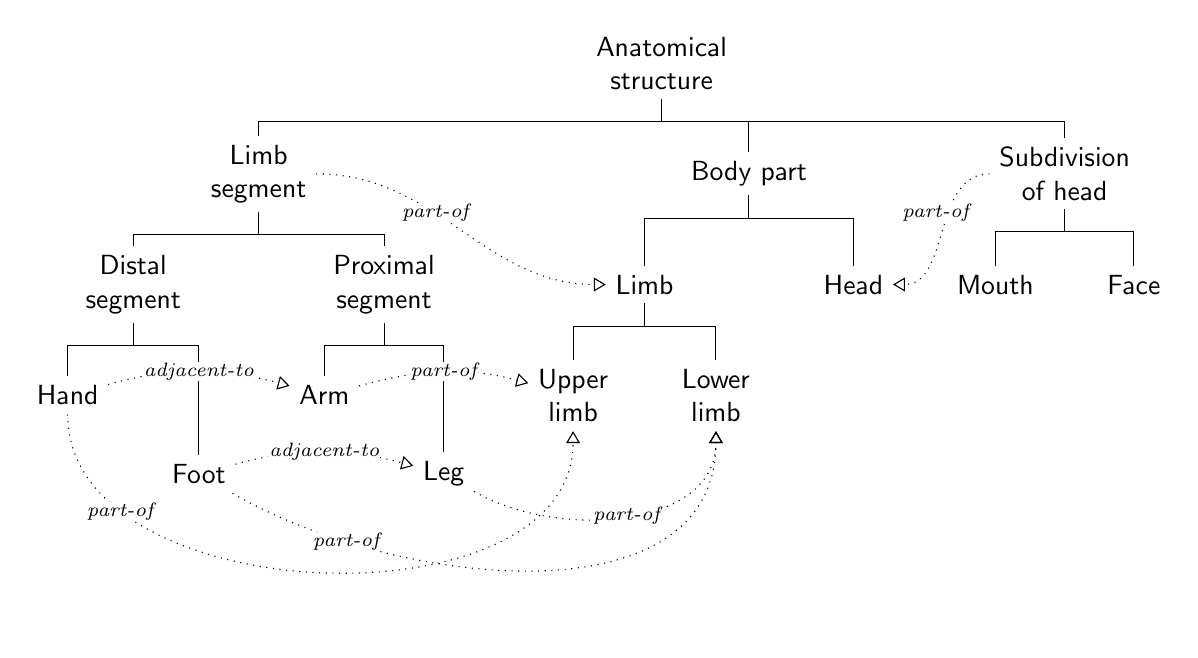
\begin{tikzpicture}[
    level distance=4em,
    sibling distance=2em,
    every tree node/.style={align=center,font=\sffamily},
    edge from parent/.append style={line width=0},
    edge from parent path={
        (\tikzparentnode.south) -- +(0,-8pt) -| (\tikzchildnode)
    },
    every edge/.append style={
        dotted,
        -{Triangle[scale=1.2,open]}
    },
    l/.style={
        fill=white,inner sep=0.1mm,node font=\scriptsize\itshape
    }
]
    \Tree [
        .\node (structure) {Anatomical\\structure}; [
            .\node (segment) {Limb\\segment}; [
                .\node (distal) {Distal\\segment};
                    \node (hand) {Hand};
                    \node (foot) [yshift=-1cm] {Foot};
            ] [
                .\node (proximal) {Proximal\\segment};
                    \node (arm) {Arm};
                    \node (leg) [yshift=-1cm] {Leg};
            ]
        ] [
            .{Body part} [
                .\node (limb) {Limb};
                    \node (upper) {Upper\\limb};
                    \node (lower) {Lower\\limb};
            ]
            \node (head){Head};
        ] [
            .\node (subdivion) {Subdivision\\of head};
                \node (mouth) {Mouth};
                \node (face) {Face};
        ]
    ]
    
    \draw (foot)
        edge [out=330,in=270] node [l,pos=0.2] {part-of}
        (lower);
    
    \draw (leg)
        edge [out=330,in=270] node [l,pos=0.5] {part-of}
        (lower);
    
    \draw (hand)
        edge [out=270,in=270] node [l,pos=0.2] {part-of}
        (upper);
    
    \draw (arm)
        edge [out=15,in=165] node [l,pos=0.5] {part-of}
        (upper);
    
    \draw (hand)
        edge [out=15,in=165] node [l,pos=0.5] {adjacent-to}
        (arm);
    
    \draw (foot)
        edge [out=15,in=165] node [l,pos=0.5] {adjacent-to}
        (leg);
    
    \draw (segment)
        edge [out=0,in=180] node [l,pos=0.4] {part-of}
        (limb);
    
    \draw (subdivion)
        edge [out=180,in=0] node [l,pos=0.4,xshift=-0.5em] {part-of}
        (head);
    
\end{tikzpicture}

\end{document}





